\subsection{Visualization of Performance Portability}

\citet{sewall_interpreting_2020} 
different visualization strategies:
\begin{itemize}
    \item Box Plots: obscures the "did not run" case (large boxes); no number of supported platforms; only median to compare in case of "did not run" (boxes cover whole range)
    \item Histograms: distribution of bins ("did not run" must be own bin; how many bins?); areas of low density $\rightarrow$ difficult to "see" the distribution
    \item Probability Density Function: primary problem choosing a good kernel bandwidth; PP sparse and uneven distributed data $\rightarrow$ no fixed bandwidth guaranteed to yield satisfactory results $\rightarrow$ adaptive methods; problems on [0, 1] boundaries $\rightarrow$ there may be many points there for PP making this problem even worse; but better than Histograms (better tendencies; less crowded bars)
    \item Violin Plots: a combination of kernel density estimation and Box Plots

    % Impact of Platform Selection
    \item plotting \pp against $\mathcal{H}$ $\rightarrow$ other paper \cite{deakin_performance_2019}
    \item Efficiency Cascade Plots + Platform Charts: minimum efficiency and H $\rightarrow$ remove platform with minimum efficiency and start again; independent for each application; platform sets at the bottom may not be the same for each application; monotonic decreasing
\end{itemize}

\todo{Plot script anpassen und für mich unnötiges Zeug rauswerfen.}
\begin{figure}
    \centering
    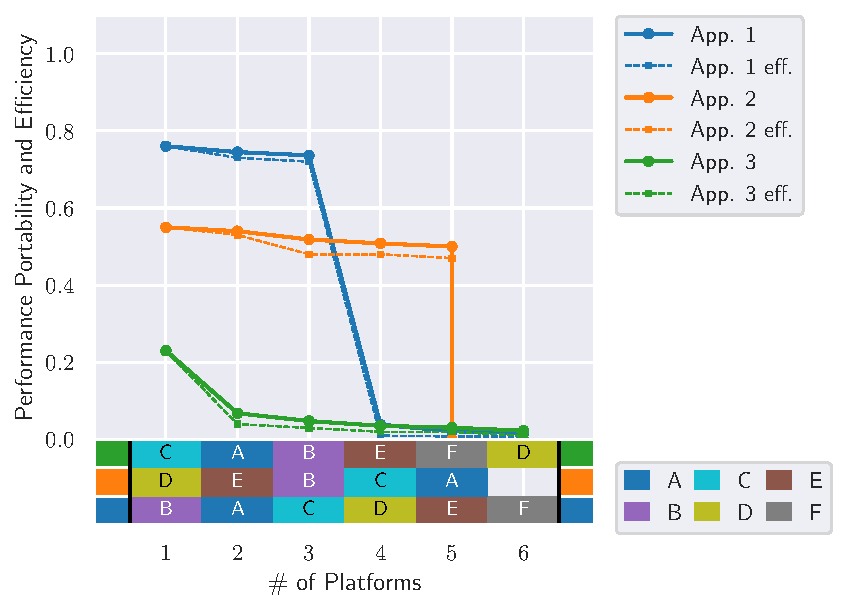
\includegraphics[width=\linewidth]{figures/02_performance_portability/example_diss_eff_cascade.pdf}
    \caption{%
    An example visualization of the performance efficiencies of \autoref{tab:platforms_example} and performance portability metrics of the two example applications from \autoref{tab:pp_app_1_example} and \autoref{tab:pp_app_2_example} as proposed by \citet{sewall_interpreting_2020}. 
    TODO: further description, falsch für \mpp?
    }
    \label{fig:pp-example-visualization}
\end{figure}